%%%%%%%% ICML 2018 EXAMPLE LATEX SUBMISSION FILE %%%%%%%%%%%%%%%%%

\documentclass{article}

% Recommended, but optional, packages for figures and better typesetting:
\usepackage{microtype}
\usepackage{graphicx}
\usepackage{placeins}
\usepackage{hyperref}
\usepackage{cleveref}
\usepackage{bm}
\usepackage{xcolor}
\usepackage{amsthm}
\usepackage{amsfonts}
\usepackage{subfigure}
\usepackage{stmaryrd}
\usepackage{booktabs} % for professional tables
\usepackage{paralist}
\usepackage{xspace}


% hyperref makes hyperlinks in the resulting PDF.
% If your build breaks (sometimes temporarily if a hyperlink spans a page)
% please comment out the following usepackage line and replace
% \usepackage{icml2018} with \usepackage[nohyperref]{icml2018} above.
\usepackage{amsmath}

% Attempt to make hyperref and algorithmic work together better:
\newcommand{\theHalgorithm}{\arabic{algorithm}}

\newcommand{\norm}[1]{\left\lVert#1\right\rVert}
\newcommand{\abs}[1]{\left|#1\right|}
\newcommand{\diag}[1]{\text{diag}\left(#1\right)}
\newcommand{\intint}[1]{\left\llbracket#1\right\rrbracket}
\newtheorem{proposition}{Proposition}[section]


% Use the following line for the initial blind version submitted for review:
\usepackage{icml2018}
\newcommand{\srm}[1]{\textcolor{red}{{\bf Sam:} #1}}
\newcommand{\tim}[1]{\textcolor{red}{{\bf Tim:} #1}}
\newcommand{\ra}[1]{\textcolor{blue}{{\bf ra:} #1}}
\newcommand{\gl}[1]{\textcolor{violet}{{\bf Gl:} #1}}
\newcommand{\mpv}[1]{\textcolor{green}{{\bf MV:} #1}}
\newcommand{\shrink}{{\bf ShrinkNets}\xspace}
\newcommand{\swl}{{\bf SwitchLayer}\xspace}
\newcommand{\swls}{{\bf SwitchLayers}\xspace}
% If accepted, instead use the following line for the camera-ready submission:
%\usepackage[accepted]{icml2018}

% The \icmltitle you define below is probably too long as a header.
% Therefore, a short form for the running title is supplied here:
\icmltitlerunning{Learning Neural Network size with ShrinkNets}

\begin{document}

\twocolumn[
\icmltitle{Learning Network Size while Training with ShrinkNets}

% It is OKAY to include author information, even for blind
% submissions: the style file will automatically remove it for you
% unless you've provided the [accepted] option to the icml2018
% package.

% List of affiliations: The first argument should be a (short)
% identifier you will use later to specify author affiliations
% Academic affiliations should list Department, University, City, Region, Country
% Industry affiliations should list Company, City, Region, Country

% You can specify symbols, otherwise they are numbered in order.
% Ideally, you should not use this facility. Affiliations will be numbered
% in order of appearance and this is the preferred way.
\icmlsetsymbol{equal}{*}

\begin{icmlauthorlist}
\icmlauthor{Guillaume Leclerc}{mit,epfl}
\icmlauthor{Raul Castro Fernandez}{mit}
\icmlauthor{Manasi Vartak}{mit}
\icmlauthor{Martin Jaggi}{epfl}
\icmlauthor{Samuel Madden}{mit}
\end{icmlauthorlist}

\icmlaffiliation{mit}{Computer Science and Artificial Intelligence Laboratories, Massachusetts Institute of Technology, Cambridge, Massachusetts, USA}

\icmlaffiliation{epfl}{Swiss Federal Institute of Technology, Lausanne, Switzerland}

\icmlcorrespondingauthor{Guillaume Leclerc}{leclerc@mit.edu}

% You may provide any keywords that you
% find helpful for describing your paper; these are used to populate
% the "keywords" metadata in the PDF but will not be shown in the document
\icmlkeywords{Machine Learning, ICML}

\vskip 0.3in
]

% this must go after the closing bracket ] following \twocolumn[ ...

% This command actually creates the footnote in the first column
% listing the affiliations and the copyright notice.
% The command takes one argument, which is text to display at the start of the footnote.
% The \icmlEqualContribution command is standard text for equal contribution.
% Remove it (just {}) if you do not need this facility.

%\printAffiliationsAndNotice{}  % leave blank if no need to mention equal contribution
\printAffiliationsAndNotice{} % otherwise use the standard text.

\begin{abstract}
As neural networks are being increasingly deployed in different applications and
on different hardware, it has become increasingly important to optimize
inference time and model size along with model accuracy.  Most current work
optimizes model size, model accuracy and inference time in different stages and
results in suboptimal results at the cost of computational inefficiency.  In
this work, we propose a new techique called ShrinkNets that optimizes all three
of these metrics simultaneously by learning optimal network size at training
time.  Specifically our technique presents a new method to simultaneously
optimize network size and model performance by neuron-level pruning.
Neuron-level pruning not only produces much smaller networks for a given
accuracy threshold but also produces dense weight matrices that are efficient at
inference time.  By applying our technique to a variety of models with both
convolutional and fully connected layers, we show that ShrinkNets can reduce by
35\% the network size with respect to a static network for \texttt{CIFAR10}, and
it can achieve speedups during inference time of up to 40X. In addition, the
most accurate networks found by ShrinkNets are similar or more accurate than
those found by statically trained networks.  
\end{abstract}

%\section{Tentative outline}
%
% \begin{itemize}
  % \item We want to figure out what is the proper network size
  % \item If we had a oversized network and for each neuron we would have an on/off switch, we could optimize the state of each switch to achieve any size/accuracy tradeof (we can prove that, do we care ?)
  % \item Solving such problem is NP-Hard
  % \item We could approximate the binary switch by relaxing them and doing L1 loss instead of L0 loss
  % \item This is the definition of Shrinknets
  % \item group sparsity tries to achieve a similar goal but with a different formulation
  % \item How are they related ?
  % \item If we add a specific constraint on our formulation we obtain the group sparsity one (proven)
  % \item We conclude that without this constraint our formulation has more degree of freedom
  % \item What happen when we drop this constraint
  % \item The problem becomes non-convex and without a global minimum
  % \item Not having a global minimum is bad, how can we solve that ?
  % \item Adding an extra regularization parameter allow us to have a global minimum (a lot of them actually)
  % \item Now we have a framework to switch on and of neurons
  % \item We are still doing useless computation for neurons that will stay off forever, if we pruned them then we would speed up training
  % \item Define the strategy to detect "forever dead" neurons
  % \item (should we talk about the software architecture ?)
  % \item now we evaluate the system
  % \item First we show that our system has indeed more freedom than Group sparsity by showing that for any given amount of sparsity it can fit closer than the previous method
  % \item On the same problem we show that removing neurons on the fly does not dramatically reduce accuracy (we might not be able to see any difference in performance for a linear/logistic regression though)
  % \item We show that works with Bigger networks (multi layers perceptrons and CNNs), describe the training dynamics, discuss the shape we obtain
  % \item Show that it is easier to do hyper-parameter optimization on the regularization parameter that the size of each layer. I think a nice experiment would be to plot the evolution of the final size of a two layer network (so going from a lambda to two sizes). And plot the trajectory in the "size space" as we decrease lambda. It would show how the system trades off the budget between the two layer in a nice and visual way
  % \item Then we evaluate performance
% \end{itemize}

% \section{Outline2}
%\begin{itemize}
%  \item Introduction
%  \begin{itemize}
%    \item Finding an appropriately sized network is challenging
%    \item ML practitioners spend a large amount of time tuning the size of layers
%    in a network in order to get the best possible accuracy.
%    \item Many techniques have been proposed for hyperparam opt but these
%    are computationally expensive and take long to train
%    \item We propose ShrinkNets, an approach to tune the size of the network 
%    as it is being trained without incurring the significant costs of 
%    hyperparameter optimization. 
%    \item Thus, our contribution are: ...
%  \end{itemize}
%  \item Our Approach
%  \begin{itemize}
%    \item Assign an on/off switch to each neuron. But this is np-hard, so we
%    consider a relaxation
%    \item Formulation
%    \item Relationship to sparsity
%    \item Strategies to kill neurons (relation to theory above?)
%    \item Implementation details
%  \end{itemize}
%  \item Related Work
%  \begin{itemize}
%    \item Hyperparameter optimization: random, bayesian opt, bandit methods
%    \item distillation techniques
%    \item post-training compression techniques
%    \item group sparsity, non-parametric neural networks
%    \item training dynamics paper: first overfitting and then randomization?
%  \end{itemize}
%  \item Experiments
%  \begin{itemize}
%    \item Accuracy obtained by Shrinknets
%    \item Time taken to reach that accuracy compared with other hyperopt methods
%    \item Characterize method wrt params
%    \item Other experiments
%  \end{itemize}
%  \item Discussion
%  \begin{itemize}
%    \item Where does the method shine?
%    \item Side-effects of method: smaller networks, time to train
%    \item Potential extensions/limitations
%  \end{itemize}
%  \item Conclusion
%\end{itemize}

%!TEX root=paper.tex

\section{Introduction}

Neural networks are increasingly being deployed in a wide variety  of
applications  and on diverse hardware architectures ranging from laptops to
phones to embedded sensors. This wide variety of deployment settings means
that inference time and model size are becoming as important as  prediction
quality when assessing model performance.  However, these three dimensions of
performance (model quality, inference time and model size)  are largely
optimized separately today, often with suboptimal results.

Of course, the problem of finding compressed or small networks is not new.
Existing techniques to make a pre-trained neural network smaller can be
categorized in two approaches: (1) quantization \cite{quant} and code
compilation~\cite{ma2016compilation}, techniques that can be applied blindly to
any network, and (2) techniches which analyze the structure of the network and
systematically prune connections or neurons~\cite{han2015deepcompression,Cun}
based on some loss function. While the first category is always useful, but only
has limited impact on the network size, the second category can reduce the model
size much more but has several drawbacks:   First, those techniques often
negatively impact model quality.  Second, they can (surprisingly) negatively
impact inference time as they transform dense matrix operations into sparse
ones, which can be substantially slower to execute on modern hardware
\cite{han2015deepcompression}, especially GPUs which do not efficiently support
sparse linear algebra.  Third, these techniques generally start by optimizing a
particular architecture for prediction performance, and then, as a post-
processing step, applying compression  to generate a smaller model that meets
the resource constraints of the deployment setting.  Because the network
architecture is essentially fixed during this post-processing,   model
architectures that work better in small settings may be missed -- this is
especially true in large networks like many-layered CNNs,  where it is
infeasible to try explore even a small fraction of possible network
configurations.

%I am still not super happy with the flow. Will work on it more. 

In contrast, in this paper we present a new method to simultaneously optimize
 network size and model performance. The key idea is to learn the right
network size at the same time that we optimize for prediction performance for a
specific task. Our approach, called {\it ShrinkNets}, starts with an {\it
over-sized} network, and dynamically shrinks it by eliminating unimportant
neurons---those that do not contribute to prediction performance---during
training time. To do this, ShrinkNets must detect the unimportant neurons, and
remove them from the network. The
removal of entire neurons and not connections is crucial, because it leads to
dense networks, which in turn leads to better inference performance. To support the
detection and removal of unimportant neurons we introduce a new layer, called
\textbf{Switch layer}. Introducing this new layer simply requires us to
add a term to the
loss function to optimize the weights of this layer during training. ShrinkNets has
two main benefits. First, it explores the architecture of models that are both
small and perform well, rather than starting with a high-performance model and
making it small.  It does this using a single new hyperparameter that effectively 
models the target network size.  This allows us to efficiently generate a family of smaller and
accurate models without an exhaustive and expensive hyperparameter search over
the number of neurons in each layer.  Second, in contrast to existing neural
network compression techniques~\cite{Aghasi2016,han2015deepcompression}, our
approach results in models that are not only small, but where the layers are
dense, which means that inference time is also improved, e.g., on GPUs.





% {\bf Old introduction:}
% One of the key defactors that affects neural net perforamnce is  is the {\it shape} of the network, 
% i.e., the number of layers, the number of neurons per layer, and the connections between
% layers.
% An {\it under-sized} network, with too few neurons or layers,
%  is likely to have low accuracy because of insufficient 
% capacity while an {\it over-sized} network is slow to train due to additional 
% parameters and is computationally inefficient at both training and inference time.
% % A sub-optimal network shape can lead to low accuracy .
% %Although the hyperparameters related wo network size can dramatically affect
% % performance, there is no reliable way to efficiently set them.
% Consequently, many {\it hyperparameter optimization} techniques have been proposed to determine the optimal size of
% a neural network; these include random search~\cite{paper-on-random-is-good-enough}, 
% what-is-this-paper~\cite{Bengio2012a}, 
% meta-gradient descent~\cite{Pedregosa2016},
% Gaussian processes~\cite{Bergstra2011a}, and many others.
% \srm{Are we really sure that no other techniques optimize the network size during training like we do?  Don't we also require 
% iterating over lambda?  Is this really the key contribution of our work, that it reduces model search time?  Isn't the key point that
% we find smaller, better models?}
% These existing techniques all require a compute-intensive search of 
% model space,  often training of tens or hundreds of models.
% As a result, tuning these techniques require times 
% longer (or many times more computational power) 
% than the time take for a single training run.

% In this paper we present a novel method to automatically find an appropriate
% network size, which drastically reduces optimization time. \srm{In comparison to previous search models?}
% The key idea is to learn the network size while optimizing the primary objective function.
% Our strategy, called \textbf{ShrinkNets}, is blah blah \mpv{Short blurb about the technique}
% % For example, for an image classification task, with our approach we can 
% % provide the training data to a network—without sizing it a priori—and expect 
% % to end up with a network that has learned to classify images with an accuracy
% % similar to a the best manually engineered network. 
% Our approach has two main benefits. 
% First, we no longer need to choose a network size before training.
% We simply set an initial size for the network and then the algorithm will
% determine the best network that is smaller or equal in size to the inital size.
% Second, this optimization is done during a {\it single} training run, as opposed to the large number of training runs
% required by existing hyperparameter optimization 
% techniques.  As a result, we can find the best model 
% faster as well as with less computational overhead.

In summary, our contributions are as follows: 

\begin{compactenum}

\item We propose a novel technique based on dynamically switching on and off neurons, 
which allows us to optimize the network size while the network is trained. 

\item We implement our technique so as to remove entire neurons, therefore
leading not only to small and well-performing networks, but also dense, which
means higher inference performance. Furthermore, our switching layers used during training can be 
savely removed before the model is used for inference, leading to zero additional overhead. 

%\item \srm{xxx postprocessing techniques to strip out switch layers}

\item We show that our technique is a relaxation of group LASSO~\cite{Yuan2006}
and prove that our problem admits many global minima.

\item We demonstrate our claims with both fully-connected and convolutional well
known neural network architectures. We show that with ShrinkNets for
\texttt{CIFAR10} we achieve the same accuracy than a traditionally trained
network while reducing the network size by a factor of $2.2x$. Further, when
willing to sacrifice only $1$\% of performance, ShrinkNets finds networks which
are 35\% smaller. All in all, this leads to speedups in inference time of up to
6x. 

%\item We demonstrate the efficacy of our technique on both convolutional and
%fully-connected neural nets, showing that ShrinkNets finds networks within
%+/-X\% of best hand-crafted accuracy in XX\% of training time compared to
%existing hyperparameter optimization methods. \srm{Mention the specific
%model/dataset where this is true.}

%\item We demonstrate that ShrinkNets can achieve this accuracy with only YY\% of
%neurons. \srm{This claim should be something about how much smaller a network
%with say 99\% accuracy is one some real dataset}
%
%\item \srm{Some claim about inference time}
%
%\item \srm{Some claim about model size vs performance}

\end{compactenum}

% The remaining of this paper is organized as follows. In section
% \ref{sec:relatedwork} we discuss the related work. In section
% \ref{sec:approach}, we introduce our approach ShrinkNets, followed by the
% practical considerations we implemented to make it work in section
% \ref{sec:impl}. Then, we evaluate the approach in section \ref{sec:evaluation}
% and conclude the paper in section \ref{sec:conclusions}.



%!TEX root=paper.tex
\section{Related Work}

%\begin{itemize}
%  \item post-training compression techniques -- brain damage , 
%  \item group sparsity e.g., \cite{Scardapane2017} and non-parametric neural networks -- 
%  \item training dynamics paper: first overfitting and then randomization?, \gl{Here is the ref, if you can introduce it in the flow \cite{Shwartz-Ziv2017}}
%\end{itemize}

There are several lines of work related to optimizing network structure. 

%Given the importance of network structure, many researchers have explored the
%problem of finding the best network structure for a given learning task.  The
%proposed techniques broadly fall into five categories: random search andbrute
%force search, hyperparameter optimization, model compression after training,
%resizing models during training, and automated architecture search methods.

\noindent\textbf{Hyperparameter optimization techniques: }
One way to optimize network architecture is to use 
hyperparameter optimization.  Although many methods have been 
proposed, e.g., \cite{BergstraJAMESBERGSTRA2012,Snoek12},
randomized search has been shown to work surprising well.
%  Brute force search of network sizes is
%also become more practical due to faster and more powerful
%hardware~\cite{molchanov2016pruning}.  
The more complex methods for
hyperparameter optimization include techniques, e.g., ~\cite{Snoek12} typically
 select hyperparameter combinations that come from uncertain areas of the
hyperparameter space to search efficiency. 
As a generalization of this,  methods based on bandit algorithms (e.g.
~\cite{li2016hyperband, jamieson2016}) have also become a popular way to tune
hyperparameters by quickly discarding 
model configurations that perform badly. 
Although these methods could in theory be used to tune the number of neurons per layer
of a network, in practice no related work proposes this, because treating each layer as a hyperparameter
would lead an excessively large search space.
In contrast, with ShrinkNets the size of the network can be tuned with 
a single parameter, as we explain in the next section..
% More importantly, none of the hyperparameter optimization methods focuses on
% finding small networks, which is a crucial property of ShrinkNets, necessary to
% achieve good inference times.

%As noted before, all of the above techniques require many tens
%to hundreds of models to be trained, making this process computationally
%inefficient and slow.  More practically, the hyperparameter optimization
%literature does not evaluate their methods on network size and instead focuses
%on optimization hyperparameters such as learning rates and weight decay
%parameters.

\noindent\textbf{Model Compression: }Model compression techniques focus on
reducing the model size \emph{after} training, in contrast to ShrinkNets, which
reduces it \emph{while} training. 
Optimal brain damage~\cite{Cun} identifies connections in a network that are
unimportant and then prunes these connections.
DeepCompression~\cite{han2015deepcompression} takes this one step further and in
addition to pruning connections, it quantizes weights to make inference
extremely efficient.  A different vein of work such as ~\cite{romero2014fitnets,
hinton2015distilling} proposes techniques for distilling a network into a
simpler network or a different model. Because these techniques work after
training, they are orthogonal and complementary to ShrinkNets. Further,
some of these techniques, e.g.,~\cite{Han2015,Cun}, produce sparse matrices that
are not likely to improve inference times even though they reduce network size.
%Unlike our technique which works during
%training, these techiques are used after training and it would be interesting to
%apply them to ShrinkNets as well. 
%\cite{Abadi2016b} share the common goal of
%removing entire blocks of parameter to maintain dense matrices, however their
%method only applies to convolutional layers.

\noindent\textbf{Auto-ML: } Some work that focuses on automatically learning
model architecture through the use of genetic algorithms and reinforcement
learning techniques~\cite{DBLP:journals/corr/ZophL16, zoph2017learning}. These
techniques are focused on learning higher-level architectures (e.g.,
building blocks for neural network architectures). In particular, they do not
focus on finding small but well-performing networks for inference, which is the
goal of ShrinkNets.

\noindent\textbf{Dynamically Sizing Networks: }The techniques closest to our
proposed method are those based on group sparsity such as
~\cite{Scardapane2017}, and those like~\cite{Philipp} that dynamically grow and shrink
 the size of the network during training.  \cite{Scardapane2017}
presents a method that also deactivates neurons using a loss function based on
group-sparsity.  However, the exact details of how their method works are not
given, and their experimental results (on a small, fully connected network), are
substantially worse than ours as shown in Section~\ref{sec:experiments}.
\cite{Philipp} propose a method called Adaptive Radial-Angular Gradient Descent
that adds neurons on the fly and removes neurons via an $l_2$ penalty.  However,
this approach requires a new optimizer and takes longer to converge compared to
ShrinkNets.




\section{Our Approach}

% from the universality theorem, we know that we can find a network that ca
% arbitrarly fit a function. Therefore, for a given error tolreance there exists
% an optimal size to solve a given problem.

Our approach is based on the insight that given enough capacity (and time), an 
optimization routine can find a network that can fit an arbitrary function.
Therefore, by starting with an oversize network and applying on/off switches to
each of the neurons in it, we can identify a {\it pruned} version of the network
that can achieve similar accuracy to the oversized network.


% If we have an oversized network then there exist a pruned version that can still
% achieve our goal. The main idea is to consider an on/off switch for each neuron,
% and we want to find an assignement for this switches that achieve a certain
% size/accuracy tradeof. 
We model these on/off switches by multiplying each input
(or output) of each layer by a number $0$ or $1$. 
$0$ will deactivate the
neuron, $1$ will let the signal go through. 
We want to minimize the number of on
switches to reduce the model size as much as we can. 
This can be modeled solved
by jointly minimizing the objective of the network and a factor of the L0 norm
of the vector containing all the on/off switches.

Finding an optimal binary assignement is an NP-Hard problem. 
% (\textbf{Should we
% prove this ? I think it should be fairly doable reducing it to 3-SAT
% considering the structure of neural networks. No.})
We relax this problem
% problem because this is what people usually do with NP-Hard problem. Our
% relaxation is we allow 
by allowing $\bm{\theta}$ to be a real number instead of a 0/1 value, thus
constraining the L1 norm as opposed to the L0 norm.
% , effectively
% t We
% also use L1 instead of L1. This way we obtain a non-convex, but at least
% differentiable (almost everywhere).

This approach assumes that we start with an upper bound on the model size. This
obviously translates in a computational overhead. Our insight is that some
usless neurons (we have multiple definitions below) can be removed early without
impacting the final solution. It has two practical implications: It mitigate the
issue we describe but it also allows other neurons to adapt as soon as one of
their peer is killed. Existing technique usually remove them after convergence
and require an extra fine-tuning process to compensate for the removal.

% The key components of the system are: The filter vectors that simulate the
% continuous on/off switches, a regularization that tries to kill neurons, the
% neuron removal strategy that detects neurons that should probably be removed,
% and the garbage collection that effectively remove dead neurons from the model,
% and the simplifaction procedure that remove the filter vector for fast
% inference.

% We will describe these components in the upcoming sections.

% \subsection{Notations}

% \par In order to avoid any potential ambiguity, in this section we will
% describe in details the mathematical notations used in this article. 
% Non-bold
% letters represent scalar values, while bold lowercase and upper case
% repectively denote vectors and matrices. 
% $\bm{A}^T$ stands for the transpose of
% the matrix $\bm{A}$. 
% Subscripts are used to index particular elements of
% vectors and matrices. 
% $\bm{x}_i$, $\bm{A}_i$, $\left(\bm{A}^T\right)_j$ and
% $\bm{A}_{i,j}$ respectively correspond to the $i^{th}$ component of $\bm{x}$,
% the $i^{th}$ row of $\bm{A}$, the $j^{th}$ column of $\bm{A}$ and the $j^{th}$
% component of the $i^{th}$ row of $\bm{A}$. 
% All the following definitions assume
% $\bm{A}$ to be an $n\times p$ matrix.  
 
% For any $l \in \left[0, +\infty\right]$ we define the norm: $\norm{\bm{A}}_l =
% \left(\sum_{i=1}^n \sum_{j=1}^p \abs{\bm{A}_{i, j}}^l\right)^{\frac{1}{p}}$. 
% For the rest of this paper and unless stated otherwise, $\bm{y}$ will represent the output of a network, $\bm{x}$ the input, $\bm{b}$ a bias, $\lambda$ regularization factors, $\Omega$ regularization methods, $\bm{\theta}$ general model parameters and $a$ will stand for any element-wise activation function. 
% The only constraint that we want to enforce is that $a(0) = 0$. 
% We use $\intint{u, v}$ to denote inteveral of integers, 
% $\bm{0}$ is the null vector (size depending on the context). 
% $\#S$ is meant to represent the cardinality of a set $S$. 
% To simplify the notation of function composition we use the following operator: 
% $g(f(\bm{x})) = (f \circ g)(\bm{x})$ and for a long sequence of functions from 
% $f_1$ to $f_n$ we use: $f_n(...f_1(\bm{x})) = \left(\bigcirc_{k = 1}^n f_k\right)(\bm{x})$.

We implement our strategy of dynamically deactivating neurons by means of a 
specialized neural network layer called the \textbf{Switch Layer}.
We first describe the key concepts and theory backing the switch layer and then
provide a brief summary of our implementation of switch layers.


\subsection{The Switch Layer}

% \textbf{Do you like the name of the layer ? Yes!}

Let $L$ be a layer in a neural network that takes an input tensor $\bm{x}$ and 
produces an output tensor $y$ of shape $\left(c \times d_1 \times \dots \times 
d_n\right)$ where $c$ is the number of neurons in that layer.
For instance, for fully connected layers, $n$=0 and the output is single 
dimensional of size $c$ (ignoring batch size for now) while for a 2-D 
convolutional layer, $n$=2 and $c$ is the number of output channels or feature 
maps.
% maps
% For instance, for fully connected layers, $n$=0 and the output is single 
% dimensional of size $c$ (ignoring batch size for now) while for a 2-D 
% convolutional layer, $n$=2 and $c$ is the number of output channels or feature 
% maps.
%  and furthermore, let the output
% of layer $l$ be a tensor of shape $\left(C \times D_1 \times \dots \times 
% D_n\right)$ where $C$ is the number of neurons in $l$.
% In the case of a fully connected layer, $C$ is the dimensionality of the output
% of the layer whereas in the case of a convolutional layer, $C$ is the number of
% feature maps and $\left(D_1 \times \dots \times D_n\right)$ is the size of those feature
% maps.

Suppose we wish to tune the size of $L$ by applying a switch layer.
A switch layer $S$ applied to the output of $L$ can be parametrized by a 
vector $\theta \in \mathbb{R}^c$ such that the result of applying $S$ to $L(\bm{x})$
is a tensor also of size $\left(c \times d_1 \times \dots \times d_n\right)$
such that: 
\begin{equation} 
S_{\theta}(L(\bm{x}))_{i,...} = \bm{\theta}_iL(\bm{x})_{i, ...}
\end{equation}
% where $\diag{\bm{\theta}}$ is a $c\times c$ matrix such that: $\forall
% 1 \leq i \leq c$, $\diag{\bm{\theta}}_{i, i} = \bm{\theta}_i$ and $0$ otherwise. 
Effectively, once passed through the switch layer, each output channel $i$ 
produced by $L$ is scaled by the corresponding $\theta_i$.
If for any $k$, if $\theta_i = 0$, the $i^{\text{th}}$ channel is multiplied by 
zero and wont contribute to any computations after the switch layer.
If this happens, we say the Switch layer has {\it deactivated} or killed the 
neuron of layer $L$ corresponding to channel $i$. 
% Switch layers have weights in the range $[-\infty,+\infty]$ and are usually 
% placed after linear and convolutional layers.
% The \textit{Switch Layer} takes an input of size $\left(B \times C \times D_1
%   \times \dots \times D_n\right)$, where $B$ is the batch size, $C$ the number
% of features (or channels, in the case of convolutional layers), and $D$ any
% additional dimension. 
% This structure makes it compatible with fully connected
% layers with $n=0$ or convolutional layers with $n=2$. 
% Their crucial property is
% a parameter $\theta \in \mathbb{R}^C$. 
% The output is defined as follows: \vspace{-1em}
% \begin{equation} 
% Switch(\bm{I};\bm{\theta}) = \diag{\bm{\theta}} \bm{I}  
% \end{equation}
% where $\diag{\bm{b}}$ a $n\times n$ matrix such that: $\forall
% 1 \leq i \leq n$, $\diag{\bm{b}}_{i, i} = \bm{b}_i$ and $0$ otherwise. 

% Where $\theta$ is expanded in all
% dimensions to match the input size (except the second one since they are equal
% by definition). 

% These disabled neurons/channels can be removed from the network
% without changing its output. 
% Before explaining how that is achieved, we explain
% next how the weights of the Switch Layer are initialized and adjusted during
% training.

\subsection{Training Procedure} 

To tune the size of a network, we place Switch Layers after each layer whose size
we wish to tune; these are typically the fully connected and convolutional layers
in a network.
Since the switch layers are adept at deactivating neurons, we start with an
oversized network (i.e. network with more capacity than required) and then use
switch layers to deactivate or kill off neurons that are unnecessary.

Formally, we can express this procedure in terms of a sparsity constraint that pushes
values in the $\theta$ vector to 0.
Given a neural network parameterized by weights $\bm{W}$ and switch layer 
parameters $\bm{\theta}$, we optimize the following ShrinkNet loss that 
augments the regular training loss with a 
regularization term for the switch parameters and another on the network weights.
\begin{equation}
  L_{SN}(\bm{x},\bm{y};\bm{W}, \bm{\theta}) = L(\bm{x}, \bm{y}; \bm{W}) +
  \lambda\norm{\theta}_1 + \lambda_2\norm{\bm{W}}_p
\end{equation}

%To train networks we need start with a substantially oversized network, then we
%insert \textit{Switch Layers}  (usually after every linear or convolutional
%layer except the last one) and we sample their weight from the
%$\text{Uniform}(0, 1)$ distribution. 
% we could train the network directly using our standard loss function, and we could achieve performance equivalent to a normal neural
% network. However, our goal is to find the smallest network with reasonable
% performance. We achieve that by introducing sparsity in the parameters of the
% \textit{Switch Layers}, thus forcing the deactivation of neurons
%. Indeed, having a negative component in the $\theta$
%parameter of the filter layer permamently disable its associated feature
%\gl{Maybe redundant ? we talked about that in the previous paragraph} . 
% To obtain this sparsity, we simply redefine the loss function:
% \begin{equation}
%   L'(\bm{x},\bm{y};\bm{W}, \bm{\theta}) = L(\bm{x}, \bm{y}; \bm{W}) +
%   \lambda\norm{\theta}_1 + \lambda_2\norm{\bm{W}}_p
% \end{equation}

% The additional term $\lambda|\max(0, \theta)|$ introduces sparsity (see Lasso
% loss~\cite{Tibshirani1996}). 
% The $\lambda$ parameter, that can take any
% positive value, adjusts how aggressively the network deactivates neurons, with
% larger values indicating more aggressive deactivation.
%  The second component of the loss increases the gradient with respect to $\theta$, thus pushing its value towards zero. Neurons with little impact
% on the original loss (gradient lower than $\lambda$), will not be able to
% compete against this attraction towards zero. Because the entries in $\theta$
% with a value of $0$ or less correspond to dead neurons, $\lambda$ effectively
% controls the number of neurons/channels in the entire network. Without the last
% term our problem sounds very similar to the Group Sparsity regularization which
% is well known in the area of linear and logistic regressions. In the next
% section we will try to undercover the relationship between these two problems,
% explain why we need this additional regularization term and what should be the
% value of $p$.

%!TEX root=paper.tex
%\subsection{Relation to Group Sparsity}
\noindent\textbf{Relation to Group Sparsity (LASSO): } ShrinkNets removes neurons,
i.e., inputs and outputs of layers. For a fully connected layer defined as:
%
\begin{equation} \label{fully_connected}
  f_{\bm{A}, \bm{b}}(\bm{x})=a(\bm{Ax + b})
\end{equation}
%
where $\bm{A}$ represents the connections and $\bm{b}$ the bias,
removing an input neuron $j$ is equivalent to having $\left(\bm{A}^T\right)_j =
\bm{0}$. Removing an output neuron $i$ is the same as setting $\bm{A}_i = \bm{0}$
and $\bm{b}_i = 0$. Solving optimization problems while trying to set entire
group of parameters to zero is the goal of group sparsity regularization
\cite{Scardapane2017}. In  any partitioning of the set of parameters $\bm{\theta}$ defining a model in $p$
groups: $\bm{\theta} = \bigcup_{i=1}^P \bm{\theta}_i$, group sparsity is defined as: 
%
\begin{equation}
  \Omega_\lambda^{gp} = \lambda \sum_{i=1}^p \sqrt{\#\bm{\theta_i}} \norm{\bm{\theta_i}}_2 \\
\end{equation}
%
\srm{define notation -- what is $\lambda$;  what is $\#\theta$, what is $\Omega$? Where does the square root come from?} \gl{This is how it is defined in the
original paper, it would require a few sentences to explain that, do really
need to do ?}
In fully-connected layers, the groups are either: columns of
$\bm{A}$ if we want to remove inputs, or rows of $\bm{A}$ and the corresponding
entry in $\bm{b}$ if we want to remove outputs. For simplicity, we focus
our analysis in the simple one-layer case. In this case, filtering outputs does
not make sense, so we only consider removing inputs. The
group sparsity regularization then becomes:
%
\begin{equation} \label{group_sparsity_regularization}
  \Omega_\lambda^{gp} = \lambda \sum_{j=1}^p \norm{\bm{\left(A^T\right)_j}}_2 \\
\end{equation}
%
Because $\forall i, \#\bm{\theta}_i = n$, \ra{is \# the general way of expressing
cardinality? why not $|x|$?,}  \gl{In europe |x| is for the abolute value, and I was using it in the notation section that someone removed, therefore there would have been a notation conflict}to make the notation simpler, we
embedded $\sqrt{n}$ inside $\lambda$.

Group sparsity and ShrinkNets try to achieve the same goal. We discuss next how
they are related to each other. First let's recall the two problems. In the context of approximating $\bm{y}$ with a linear regression from features $\bm{x}$), the
original ShrinkNet problem is 
%
\begin{equation}
  \min_{\bm{A}, \bm{\beta}} \norm{\bm{y} - \bm{A}\diag{\bm{\beta}}\bm{x}}_2^2 + \lambda \norm{\bm{\beta}}_1
\end{equation}
%
And the Group Sparsity problem is:
%
\begin{equation}
  \min_{\bm{A}} \norm{\bm{y} - \bm{A}\bm{x}}_2^2 + \Omega_\lambda^{gp}
\end{equation}
%

We can prove that under the condition: $\forall j\in \intint{1, p},
\norm{\left(\bm{A}^T\right)_j}_2 = 1$ the two problems are equivalent
(\cref{gps_equivalence}, see Apendix). However if we relax this constraint then ShrinkNets
becomes non-convex and has no global minimum
(\cref{unconstrained_non_convex,unconstrained_shrinknet_no_min}, also in Appendix). Fortunately,
by adding an extra term to the ShrinkNet regularization term we can prove that:
%
\begin{equation}
  \min_{\bm{A}, \bm{\beta}} \norm{\bm{y} - \bm{A}\diag{\bm{\beta}}\bm{x}}_2^2 + \Omega_\lambda^s + \lambda_2\norm{A}_p^p
\end{equation}
%
has global minimums for all $p>0$ (\cref{shrinknet_regularized_minimum}).
This is the reason we defined the \textit{regularized ShrinkNet penalty} above
as:
%
\begin{equation}
  \Omega_{\lambda, \lambda_2, p}^{rs} = \lambda\norm{\bm{\beta}}_1 + \lambda_2\norm{\bm\theta}_p^p
\end{equation}
%
In practice we observed that $p=2$ or $p=1$ are good a choice; note that the latter
will also introduce additional sparsity into the parameters because the $L_1$ is, 
thest best convex approximation of the $L_0$ norm.




\subsubsection{Neuron killing}
Once Switch layers are placed in a network and
initialized (sampled from the $\mathcal{N}(0, 1)$ distribution),

\textbf{Threshold strategy}:  We kill neurons based on a threshold (in absolute
value), this is the method used by deep compression. It is bad because it is
scale dependant and is not robust to noise in the gradients (explain that)
\\ \textbf{Sign change strategy}:  We look at when the sign change. This is also
sensitive to noise but has the advantage
\textbf{Sign variance strategy}: We measure the variance of the sign ($-1, 1$) of each component in the \textit{Switch Layer}, and consider it dead when it goes over a predefined threshold. \gl{Maybe we should add some intuition on why it makes sense}. \gl{We should probably explain the impact of $\gamma$ and report numbers from the expertiment that show that it does not hurt too much to kill neurons, we have the data in this experiment in the evaluation that we probably want to remove later.}

\subsection{Implementation}

We have implemented \textbf{Switch Layers} and the associated training procedure
as a library in pytorch~\cite{paszke2017automatic}. \gl{This is not a github citation but this is what they ask to cite}
The layer can be freely mixed with other popular layers such as convolutional
layers, batchnorm layers, fully connected layers etc.
There are two key challenges that must be overcome while implementing 
\textbf{Switch Layers}.
First, since ShrinkNets kill off a large fraction of neurons, we must remove the
overhead of carrying around dead neurons.
And second, we must update the various network layers and training machinery (e.g.
optimizer state) to reflect the deactivation of neurons.
We address these challenges by augmenting every layer with additional information
about neuron status and implementing a \emph{neural garbage collection} 
mechanism which prunes deactivated neurons on-the-fly and updates the state of 
the training machinery.
% We do so by augmenting every layer with additional information such as what
% neurons have been deactivated.
% The layer then updates its size accordingly and this change is then propagated
% to other parts of the training machinery including the optimizer which must
% know the sizes of parameters.

A second implementation challenge we address with ShrinkNets is the potentially
higher inference time.
This increase in inference time is both due to the extra computation introduced 
by switch layers and because our switch layers are not currently optimized for 
CUDA.
Therefore, for now, our library provides a post-training routine to ``fold''
switch layers into existing, optimized layers.
Specifically, for every switch layer, we check if the parent or child of this 
layer is a linearly scalable layer (e.g. convolutional layer, fully connected layer,
batchnormalization layer) and if so, we fold the switch layer into this 
neighboring layer by multiplying through by the switch weights.
In the unlikely case that a switch layer is sandwiched between two non-linearly
scalable layers, we leave the switch layer as is.


% \subsection{Speeding up training}

% In order to have a practical implementation of ShrinkNets it is absolutely
% necessary to prune useless neurons as quick as possible. In order to try more
% different strategies we split this task in two subproblems: detecting
% potentially non-crucial neurons and setting their corresponding entry in the
% switch layer to exactly 0, and neural garbage collection that 



% In our library we implemented a variant of the second strategy and the last one.

% \subsubsection{Neural garbage collection}




% It is possible to reduce the overhead of the training process by removing
% neurons as soon as they become deactivated by $\theta$ going to 0.
%If
%disabled neurons are not quickly removed, the overhead might cause the training
%process to be significantly slower than classic neural networks. 
% To do this, we implemented a \emph{neural garbage collection} mechanism which
% prunes deactivated neurons on-the-fly,  reducing the processing time
% and memory overhead. 
% To support this feature, it is crucial to understand the
% information flow between neurons and layers in the neural network. 
% We achieve
% this by representing such information flow as a graph. 
% Vertices represent layers,
% and edges are event-hubs responsible for propagating information about disabled
% neurons to the relevant layers. 
% As soon as a layer receive an event, it updates
% his parameters to reflect the new size. 
% Each operation is stored in a log that
% is used later to update other component of the system. 
% For example some
% optimizers like Adam [Ref] store state about each parameter, their state needs
% to be updated the exact same way and at the exact same time as layers in order
% to obtain apropriate parameter updates.

% \subsubsection{Speeding up Inference}
% \mpv{This may be moved to discussion or ``other considerations'' or impl details.}



% our post-processing code searches the 
% network graph to identify a parent or child layer the linear layer closest (child or parent) to every 
% switch layer and multiplies the weights of that layer by the corresponding
% switch layer weights.


% Our proposed \textit{Switch Layer} are relevant only during training, and can be
% removed from the network architecture during inference if they can be ``folded''
% into the nearest linear layer.
% Specifically, we provide a post-processing routine that will, for each switch 
% layer, search the network graph 

% The sole puropose of \textit{Switch Layer} are to detect which neurons should be
% killed and which should be left. When the training is over we will never remove
% more neurons. Therefore, they loose all their interest at inference time. 
% To
% improve size and inference time we propose the following method to get rid of
% them without changing the output of the model (modulo floating point errors).
% The basic idea is to start from every \textit{Switch Layer} and try to find the
% nearset linear operator (child or parent) and multiply its weights by the values
% in the switch layer. For example we can merge Filter layers with surrounding
% Convolutional layer, Linear layer or even BatchNormalization [ref] if they are
% before the \textit{Switch Layer}. However we need to be extremely careful not to
% cross a non-linearity otherwise it would change the output of network.
%!TEX root=paper.tex

\section{ShrinkNets in Practice}

In this section we discuss practical aspects of ShrinkNets, including the
neuron removal  process and several additional optimizations.

%The previous section described the switch layers, which deactivate neurons
%on-the-fly. To benefit from ShrinkNets in practice, we must overcome two
%challenges. First, to effectively reduce the network size we must remove the
%deactivated neurons. Since removed neurons will no longer contribute to
%improving prediction accuracy, we must be confident when removing them. Second,
%for inference, we must remove the switch layers from the network. We describe
%our solution for both challenges in this section.

\subsection{On-The-Fly Neuron Removal}
\label{neuron_killing}

Switch layers are initialized with weights sampled from $\mathcal{N}(0,1)$;
their values change as part of the training process so as to switch \emph{on}
or \emph{off} neurons. When neurons are deactivated by switch layers, we need
to remove them to actually shrink the network size. Since after removing a
neuron it will no longer be able to contribute to  prediction accuracy, we
must devise strategies that remove neurons while remaining robust to changing
values. We observe three strategies:


\textbf{Threshold strategy}: Under this strategy neurons are removed based on
a fixed threshold expressed in terms of its absolute value. This is the method
used by deep compression \cite{}. We found this method is not robust to noise
in the gradients---which occurs commonly when training networks with
stochastic gradient descent---because the threshold depends on the scale of
each weight.

\textbf{Sign change strategy}: Under this strategy neurons are removed when
the weight value changes its sign. This strategy works well in practice but it
is also sensitive to gradient noise. \ra{explain what's the consequence of
that} If we sample the gradient in a way that is not fully representative of
the dataset we might  experience one-time zero crossing which could wrongly
kill a neuron.


\textbf{Sign variance strategy}: Instead of killing  on the first zero
crossing, we can instead measure the exponential moving variance of the sign
($-1, 1$) of each parameter in the \textit{switch layer}. When the value of
the exponential moving variances goes over a predefined threshold, we consider
the neuron deactivated, and therefore we remove it. This strategy introduces
two extra parameters, one to control the behavior of the inertia of the
variance, and the threshold, but we have found it is the best performing in
practice.

The last two strategies perform better than the threshold strategy.  Both
effectively allow us to shrink the network by varying $\lambda$, and result in
networks that are both small and perform well.

%According to our experiments on linear and logistic regressions the
%two last strategies reduce the number of parameter update performed during
%training by at least an order of magnitude with only minimal impact on the final
%error obtained by the model.

\subsection{Additional Optimizations for ShrinkNets}

\noindent\textbf{Preparing for Inference: } With ShrinkNets we obtain reduced-
sized networks during training, which is the first steps towards faster
inference. This networks are readily available for inference. However, because
they include switch layers---and therefore more parameters---they introduce
unnecessary overhead at inference time. To avoid this overhead, we reduce the
network parameters by combining each switch layer with its respective network
layer by multiplying the respective parameters before emitting the final
trained network.   \ra{can't we just simply prevent the following problem at
network design time?}In the unlikely case that a switch layer is sandwiched
between two non-linearly scalable layers, we leave the switch layer as is.

\noindent\textbf{Neural Garbage Collection: }ShrinkNets decides on-the-fly
which neurons to remove. Since ShrinkNets removes a large fraction of neurons,
we must dynamically resize the network at runtime to not unnecessarily impact
network training time. We implemented a neural garbage collection method as
part of our library which takes care of updating the necessary network layers
as well as updating optimizer state to reflect the neuron removal.


%\ra{move to eval:implementation, retrieve the neuran garbace collection and
%place it somewhere here}
%We have implemented \textbf{Switch Layers} and the associated training procedure
%as a library in pytorch~\cite{paszke2017automatic}.  The layer can be freely
%mixed with other popular layers such as convolutional layers, batchnorm layers,
%fully connected layers etc.  There are two key challenges that must be overcome
%while implementing \textbf{Switch Layers}.  
%First, since ShrinkNets kill off a
%large fraction of neurons, we must remove the overhead of carrying around dead
%neurons.  And second, we must update the various network layers and training
%machinery (e.g.  optimizer state) to reflect the deactivation of neurons.  We
%address these challenges by augmenting every layer with additional information
%about neuron status and implementing a \emph{neural garbage collection}
%mechanism which prunes deactivated neurons on-the-fly and updates the state of
%the training machinery.

%A second implementation challenge we address with ShrinkNets is the potentially
%higher inference time.  This increase in inference time is both due to the extra
%computation introduced by switch layers and because our switch layers are not
%currently optimized for CUDA.  Therefore, for now, our library provides a
%post-training routine to ``fold'' switch layers into existing, optimized layers.
%Specifically, for every switch layer, we check if the parent or child of this
%layer is a linearly scalable layer (e.g. convolutional layer, fully connected
%layer, batchnormalization layer) and if so, we fold the switch layer into this
%neighboring layer by multiplying through by the switch weights.  
%In the unlikely
%case that a switch layer is sandwiched between two non-linearly scalable layers,
%we leave the switch layer as is.


%!TEX root=paper.tex
\section{Evaluation}

The goal of our evaluation is to explore (1) whether, by varying $\lambda$,
\shrink can efficiently explore (in terms of number of training runs)  the
spectrum of high-accuracy models from small to large, on both CNNs and fully
connected networks.  Our results show that, for each network size, we obtain
models that perform as well or better than \textit{Static Networks}, trained via
traditional hyperparameter optimization;  (2) whether, because these  smaller
networks are dense, they result in improved inference times on both CPUs and
GPUs; and (3) whether the \shrink approach results in network architectures that
are substantially different than the best network architectures (in terms of
relative number of neurons per layer) identified in the literature.

\noindent\textbf{Implementation: }We implemented \swls and
the associated training procedure as a library in
pytorch~\cite{paszke2017automatic}. The layer can be freely mixed with other
popular layers such as convolutional layers, batchnorm layers, fully connected
layers, and used with all the traditional optimizers. We use our implementation
to evaluate \shrink throughout the evaluation section.

\subsection{Can \shrink achieve good accuracy?}
%\subsection{Performance vs. Traditional Methods}

To answer this question we compare \shrink with a traditional network. In both
cases, we need to perform hyperparameter optimization to explore different
network architectures. We perform random search, which is an effective technique
for this purpose \cite{BergstraJAMESBERGSTRA2012}. We evaluate \shrink on two
well-known datasets. One for which it is not possible to explore the entire
space of network architectures (\texttt{CIFAR10}) and one for which it is
possible to do so (\texttt{COVERTYPE}).

\noindent\textbf{Setup: } We assume no prior knowledge on the optimal batch
size, learning rate, $\lambda$ or weight decay ($\lambda_2$). Instead, we
trained a number of models, randomly and independently selecting the values of
these parameters from a range of reasonable values. Training is done using
gradient descent and the \textit{Adam} optimizer
\cite{DBLP:journals/corr/KingmaB14}. Specifically, we start with randomly
sampled learning
rate; for every $5$ epochs of non-improvement in validation
accuracy we divide the learning rate by $10$. We stop training after $400$
epochs or when the learning rate is under $10^{-7}$, whichever comes first. For
each of the models we trained, we pick the epoch with the best validation
accuracy and report the corresponding testing accuracy. Because of the nature of
our method, it can happen that for networks that are aggressively compressed,
the best validation accuracy is obtained early in training, before the size has
converged. To be sure that accuracy measured corresponds to the final shape and
not the starting shape, we only consider the second half of the training when
picking the best epoch. For each model, we also measure the total size, in terms
of number of floating point parameters, excluding the \swls because as described
in \cref{neuron_killing}, these are eliminated after training.


\subsubsection{Large Network Setting: \texttt{CIFAR10}}


\texttt{CIFAR10} is an image classification dataset containing $60000$ color
images $(3 \times 32 \times 32)$, belonging to $10$ different classes. We use it
with the \texttt{VGG16} network \cite{Srivastava2014}, which consists of
alternating convolutional layers and \textit{MaxPool} layers interleaved by
\textit{BatchNorm} \cite{DBLP:journals/corr/IoffeS15} and \textit{ReLU}
\cite{Nair2010} layers. The two last layers are fully connected layers
separated by a \textit{ReLU} activation function.

We applied \shrink to the VGG16 network by adding \swls
after each \textit{BatchNorm} layer and each fully connected layer (except the
last). Recall that \shrink assume that the starting size of the network is
an upper bound on the optimal size. Thus, we started with a
network with 2x the recommended size for each layer as an upper bound (this
is larger than what ImageNet uses). 

We compare against classical (\textit{Static}) networks. In such networks, the
number of parameters that control the size is large: 13 parameters for the
convolutional layers and $2$ for the fully connected layers. \shrink
effectively fuse all these parameters in a single $\lambda$, but in conventional
architectures where all of these parameters are free, it is infeasible to obtain
a reasonable sample of a search space of this size. For this reason, we rely on
the conventional heuristic that the original VGG architecture (and many CNNs)
use, where the number of channels is doubled every after \textit{MaxPool} laxer.
For \textit{Static Networks} we sample the size between $0.1$ and $2$ times the size
original one, optimized for ImageNet. We report the same numbers as we did for
\shrink and we compare the two distributions. 

The results are shown in the top figure of \cref{figure_CIFAR10}, with blue dots
indicating models produced by \shrink and orange dots indicating static networks. 
For each
model, we plot its accuracy and model size. The lines show the Pareto frontier
of models in each of the two optimization settings. \shrink explore the
trade-off between model size and accuracy more effectively. 

Note that the best performing \shrink model has $92.07\%$ accuracy which
is identical to the accuracy of the static network, while the \shrink model
is $2.22$ times smaller. In addition, if we give up just 1\% error, \shrink
find a model that is 35.5 times smaller than any static network that performs
as good or better.

\subsubsection{Small Network Setting: \texttt{COVERTYPE}}

The \texttt{COVERTYPE} \cite{Blackard:1998:CNN:928509} dataset contains $581012$
descriptions of geographical area (elevation, inclination, etc...) and the goal
is to predict the type of forest growing in each area. We picked this dataset
for two reasons. First it is simple, such that we can reach good accuracy with
only a few fully-connected layers. This is important because we want to show
that \shrink find sizes as good as \textit{Static Networks}, even if
we are sampling the entire space of possible network sizes. Second, Scardapane
et al~\cite{Scardapane2017} perform their evaluation on this dataset, which
allows us to compare the results obtained by our method with the method in
~\cite{Scardapane2017}.

%The experimental setup on this dataset is similar to {\tt CIFAR10}. 
We compare \shrink against the same architecture
used in \cite{Scardapane2017}, i.e., a three fully-connected layers network with no
\textit{Dropout} \cite{Srivastava2014} and no \textit{BatchNorm}. 
%\gl{Should we say
%here that we don't expect Dropout to work here ? I could write an entire
%paragraph about it if needed}. 
In this case, for the \textit{Static Networks}, we independently sample the
sizes of the three different layers to explore all possible architectures.

The results are shown in the top figure of \cref{figure_COVER}, with the two
optimization methods plotted as before. Here, {\it Static} method finds models
that perform well at a variety of sizes, because it is able to explore the
entire parameter space.  This is as expected;  the fact that \shrink perform
as well as the Static indicates that \shrink are doing an effective job of
exploring the parameter space using just the single $\lambda$ parameter.

Note that the best performing \shrink models has $96.91\%$ accuracy while the
best static model is only $96.66\%$ accurate, while the \shrink shrink model is $2.51$
times smaller. In addition, if we give up just 0.5\% error, \shrink find a
model that is 38.6 times smaller than any static network with equivalent accuracy.


\subsubsection{Summary}

We  demonstrated that it is possible to achieve networks with good accuracy
when using \shrink both when the network space cannot be explored entirely
(\texttt{CIFAR10}) and when it can, e.g., \texttt{COVERTYPE}. The most important
result is not that \shrink find networks of good accuracy, but that those
networks are much smaller than those found by a static method. The impact of the
network size on inference time is the subject of our next evaluation goal.


\subsection{Can ShrinkNets speed up inference?}

The previous experiment showed that \shrink find networks of similar or better accuracy
than static networks that are much smaller. We now explore if the reduction in size
translates into an improvement of the inference time.

As noted in the introduction, for some applications, compact models that offer
fast inference times are as important as absolute accuracy. 

%This observation motivates our 
% the experiment approach described in the previous section 
% and shown in the top of Figure~\ref{figure_CIFAR10} 
% and~\ref{figure_COVER}:
% for a  desired target accuracy, the Pareto optimal line shows the smallest
% network
% that satisfies achieves a given accuracy. 

In this section, we study the relationship between accuracy, network size and
inference time.  To do this, we select the smallest model that achieves a given
accuracy for the both \shrink and Static approach.  For each model, we measure
the time to run inference with the model.  We then compute the ratio of the
network size and inference time between \shrink and Static at each accuracy
level, and plot them on the bottom of Figure~\ref{figure_CIFAR10}
and~\ref{figure_COVER}.  We limit our plots to the models with $80-100\%$
accuracy range because those are the ones that we consider to be practically
useful.

The middle plot in each figure shows the ratio of model size between \shrink
and Static (values $>$1 mean \shrink are smaller) at different accuracy levels.
These figures show that is that size improvements are are particularly
significant for  \texttt{CIFAR10}. In the range of accuracies we are interested
in, improvements in size go from 4x to 40x. On the \texttt{COVERTYPE} dataset,
the compression ratio is always above 1 but it rarely exceeds 3x, except for
very high accuracies where \shrink find excellent, small solutions.  The fact
that the  \texttt{COVERTYPE} networks are not dramatically smaller is expected:
as the distribution at the top of Figure~\ref{figure_COVER} shows, the static
method is able to explore most of the parameter search space, so finds a range
of models that perform well at different sizes.

For speedup, we experimented with both CPUs and GPUs, and with different batch
sizes, where batch size indicates the number of inputs simultaneously fed to the
model for inference.  For each data set/GPU/CPU combination, we show results
with batch size 1, as well as with a batch size large enough to fully utilize
the hardware on each dataset and hardware configuration.  For example, for {\tt
CIFAR10} on CPU, a batch size of 64 fully utilizes the CPU, whereas a GPU can
execute many more models in parallel, so we use a larger batch size of 1024.
For {\tt COVERTYPE}, because the model is so much smaller, larger batches are
needed to fully utilize the hardware.  Note that when using a batch size of $1$
on GPU, we do not expect to (and do not) observe any improvement because
inference times are very small (typically about 10 $\mu s$), such that setup
time dominates overall runtime.  

The bottom four graphs in each figure show the results.  Again, the {\tt
CIFAR10} results show the benefit of the \shrink approach most dramatically.  On
CPU, speedups range up to 6x depending on the batch size, with many models
exceeding 3x speedup. In general, speedups are less than compression ratios, due
to overheads in problem setup, invocation, and result generation  in
Python/PyTorch.  On GPU, the speedups are less substantial because the CUDA
benchmarking utility that we use for evaluation can choose better algorithms for
larger matrices which masks some of our benefit, although they are still often
1.5x--2x faster for large batch sizes.  The speedup results on {\tt COVERTYPE}
are similar to those for network size:  because the networks are not much
smaller, they are not much faster either.

A key takeaway of these speedup results is that, unlike local sparsity
compression methods, our methods' improvement on size translates directly to
higher throughput at inference time~\cite{Han2015}.


\begin{figure*}[t]\centering
\begin{minipage}{2.7in}
\centering
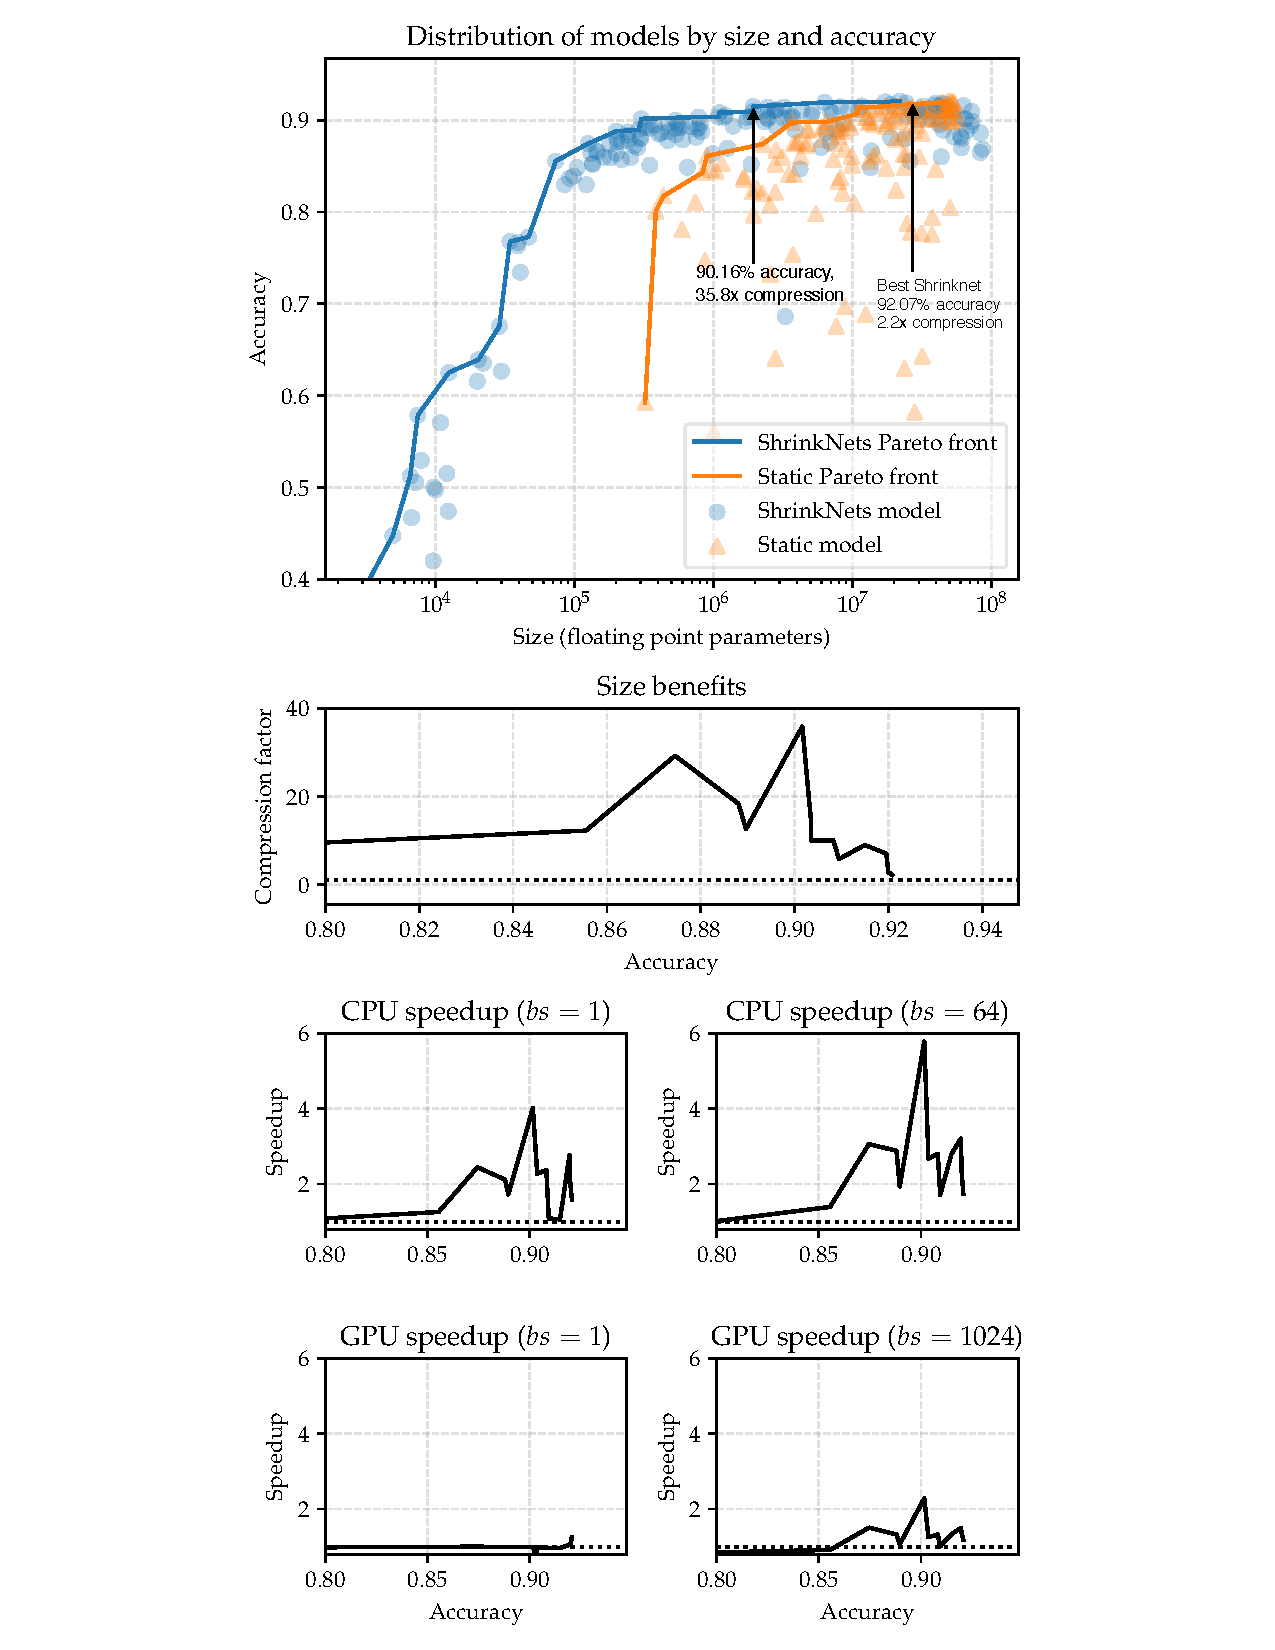
\includegraphics[width=\columnwidth]{CIFAR10_VGG_summary-arrows}
\vspace*{-10mm}
\caption{\label{figure_CIFAR10} Summary of the result of random
search over the hyper-parameters the \texttt{CIFAR10} dataset}
\vspace*{-5mm}
\end{minipage}
\begin{minipage}{.3in}
~~
\end{minipage}
\begin{minipage}{2.7in}
\centering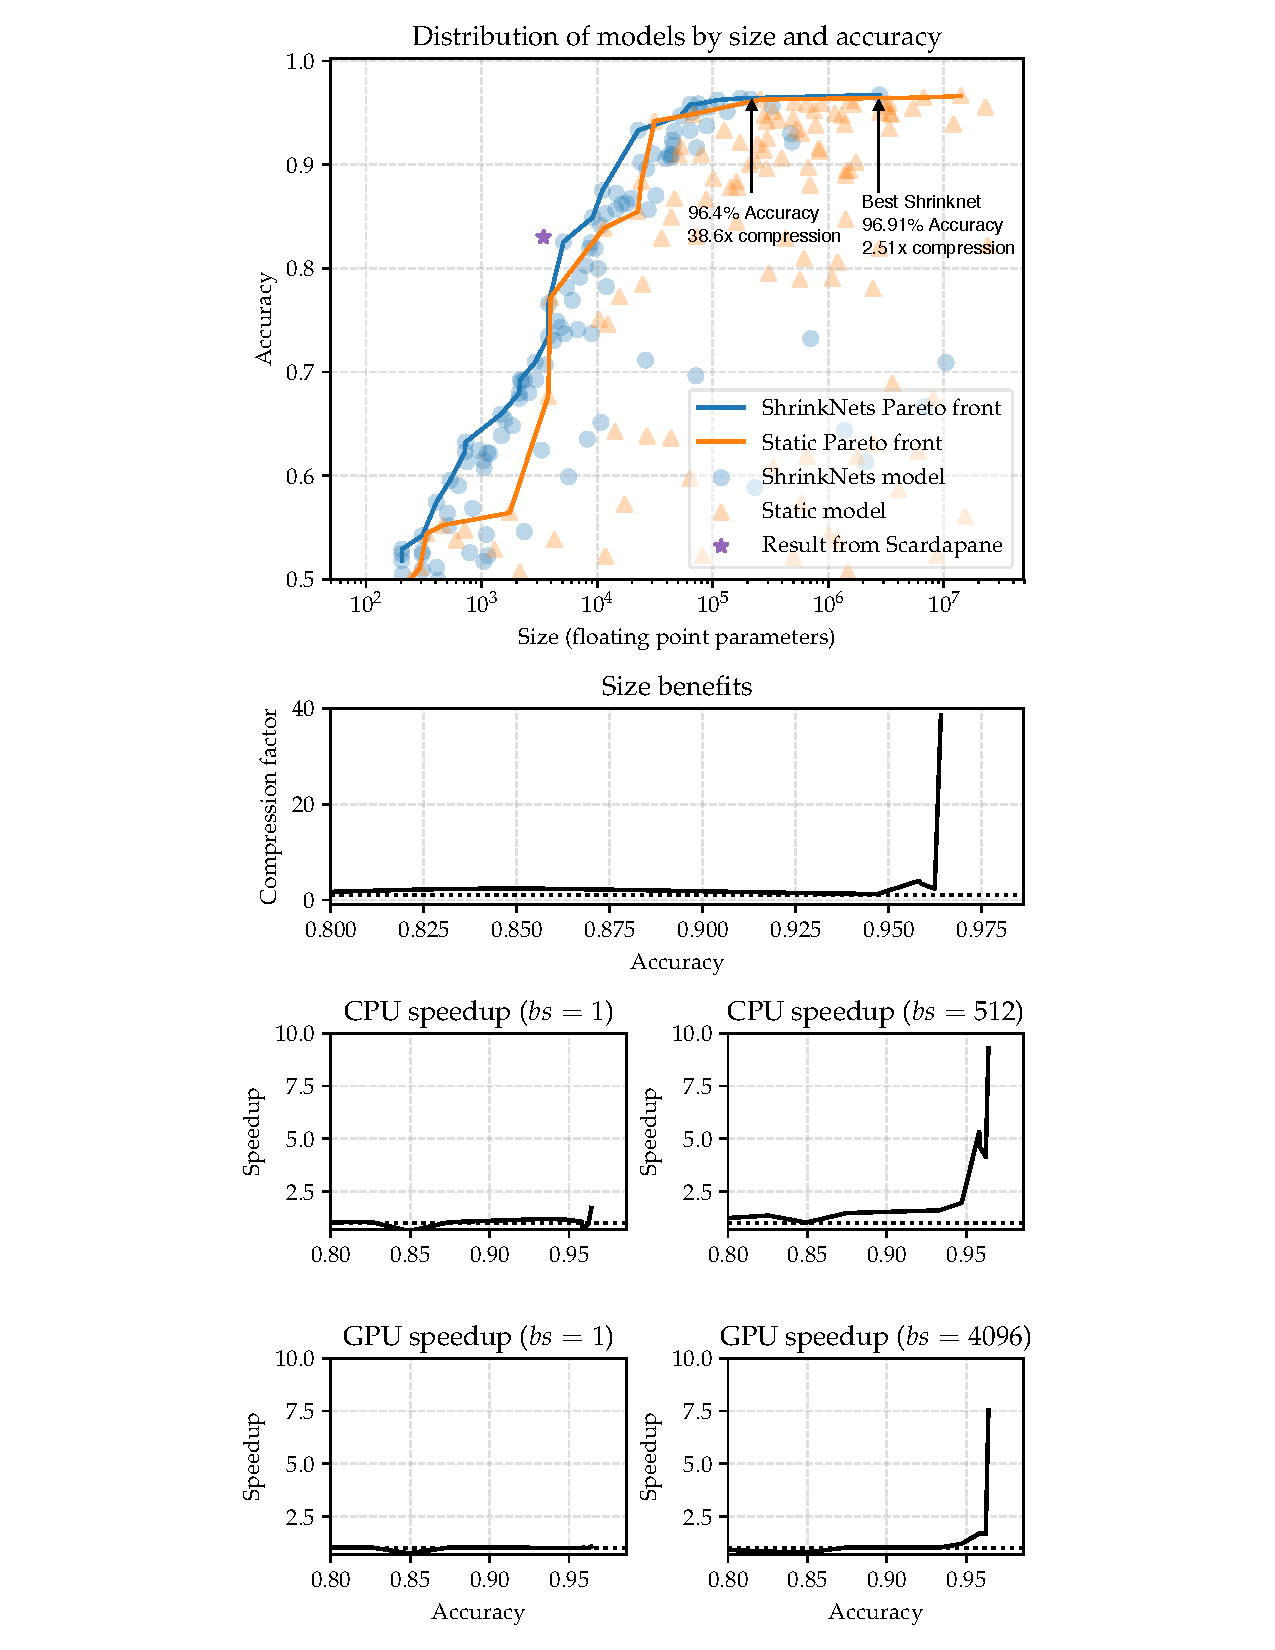
\includegraphics[width=\columnwidth]{COVER_FC_summary-arrows}
\vspace*{-10mm}
\caption{\label{figure_COVER} Summary of the result of random
search over the hyper-parameters the \texttt{COVERTYPE} dataset
}
\vspace*{-5mm}
\end{minipage}
\end{figure*}


\begin{figure}[htb]
\begin{center}
\vspace{-.1in}
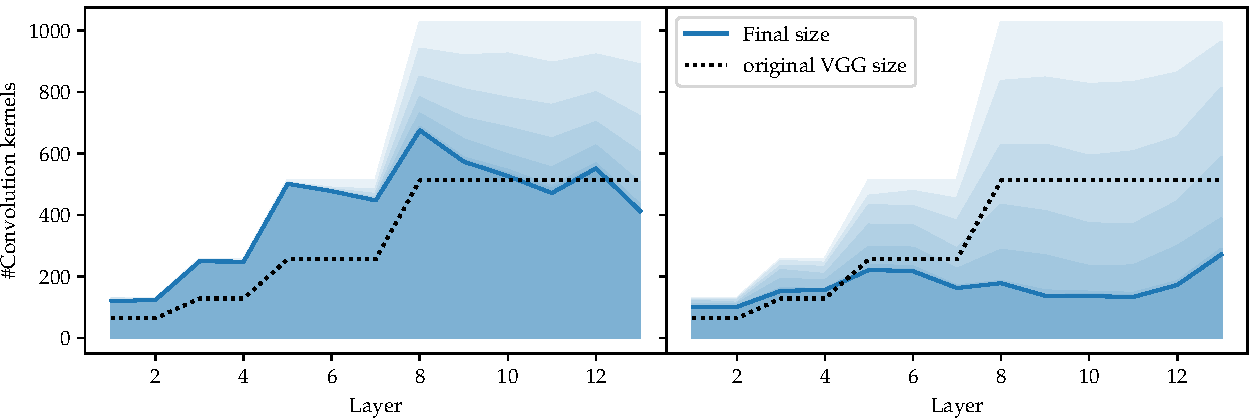
\includegraphics[width=.6\columnwidth]{size_evolution}
\vspace*{-5mm} 
\caption{ Evolution of the size of
  each layer over time (lighter: beginning, darker: end). On top a very large
  network performing $92.07\%$, at the bottom a simpler model with $90.5\%$
  accuracy. 
} 
\label{fig:network_size_evolution}
\end{center}
\vspace*{-4mm}
\end{figure}

\subsection{Architectures obtained after convergence}
\shrink effectively explore the frontier of model size and accuracy. For a
given target accuracy, the size needed is significantly smaller than when we use the
"channel doubling" heuristic commonly used to size convolutional neural networks.
This suggests that this conventional heuristic may not in fact be optimal,
especially when looking for smaller models.  Empirically we observed this to
often be the case.  For example, during our experimentations on the
\texttt{MNIST} \cite{Lecun1998} and \texttt{FashionMNIST} \cite{Xiao2017}
datasets (not reported here due to space constraints), we observed that even
though these datasets have the same number of classes, input features, and
output distributions, for a fixed $\lambda$ \shrink converged to
considerably bigger networks in the case of \texttt{FashionMNIST}. This evidence
shows that optimal architecture not only depends on the output distribution or
shape of the data but actually reflects the dataset.  This makes sense, as
\texttt{MNIST} is a much easier problem than \texttt{FashionMNIST}.

To illustrate this point on a larger dataset, we show two examples of
architectures learned by \shrink in
Figure~\ref{fig:network_size_evolution}.  The right arrow shows the model with the
best test accuracy, with identical performance to the best static
network; the left arrow shows a network that slightly under-performs the best in
terms of accuracy but is significantly smaller that the best equivalent
\textit{Static Network}.  In the plot, the dashed line
shows the number of neurons in each layer of the original VGG net, and the
shaded regions show the size of the \shrink as it converges (with the darkest
region representing the fully converged network).  Observe that the final
network that is trained looks quite different in the two cases, with the optimal
performing network appearing similar to the original VGG net, whereas the
shrunken network allocates many fewer neurons to the middle layers, and then
additional neurons to the final fewer layers.



%\section{Discussion}

\begin{itemize}
  \item Where does the method shine?
  \item Side-effects of method: smaller networks, time to train
  \item Potential extensions/limitations
\end{itemize}
%!TEX root=paper.tex
\section{Conclusion}

We presented \shrink, an approach to learn deep network sizes while training.
\shrink employs a \swl, which deactivates neurons, as well as
of a method to remove them, which reduces network sizes, leading to faster
inference times. We demonstrated these claims on on two well-known datasets, on
which we achieved networks of the same accuracy as traditional neural
networks, but up to 35X smaller, with inference speedups of up
to 6X.



\appendix
%!TEX root=paper.tex
\section{Appendix}

\begin{figure}[t]
\begin{center}
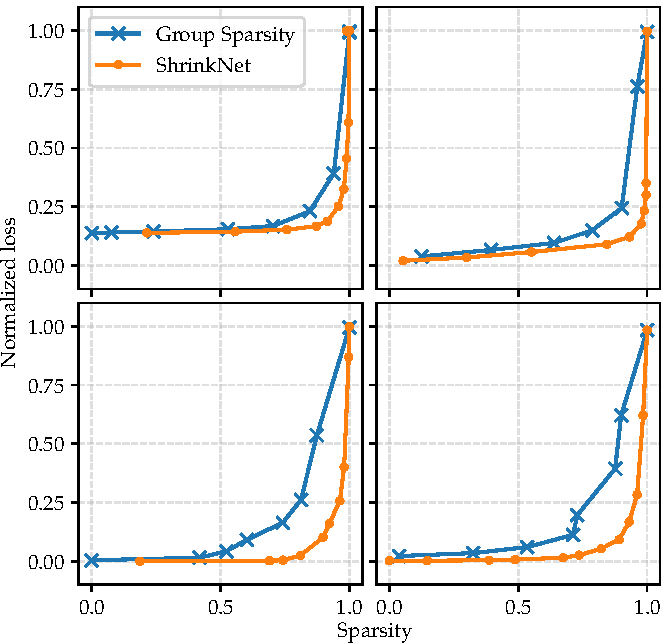
\includegraphics[width=.7\columnwidth]{regressions}
\vspace*{-5mm}
\caption{\label{sparsity_accuracy}Loss/Sparsity trade off comparison between Group Sparsity and Shrinknet on linear and logistic regression. From top to bottom and left to right we show the results for \texttt{scm1d}, \texttt{oes97}, \texttt{gina\_prior2} and \texttt{gsadd}.}

\end{center}
\vspace*{-4mm}
\end{figure}

\subsection{Proofs}
Unless specified, all the proofs consider the Multi-Target linear regression problem
\begin{proposition}
\label{gps_equivalence}
  $\forall (n, p) \in \mathbb{N}_+^2, \bm{y} \in \mathbb{R}^{n}, \bm{x} \in \mathbb{R}^{p} \lambda \in \mathbb{R}$
  
  \begin{align*}
    & \min_{\bf{A}} \norm{\bf{y} - \bf{A}\bf{x}}_2^2 + \lambda \sum_{j=1}^p \norm{\left(A^T\right)_j}_2 \\
     = &\min_{\bf{A'}, \bm{\beta}} \norm{\bf{y} - \bf{A'}\diag{\bm{\beta}}\bf{x}}_2^2 + \lambda \norm{\bm{\beta}}_1 \\
     & \text{s.t.} \forall j \in \intint{1, p}, \norm{\left(A'^T\right)_j}_2^2 = 1
  \end{align*}
\end{proposition}

\begin{proof}
  In order to prove this statement we will show that for any solution $\bm{A}$ in the first problem, there exists a solution in the second with the exact same value, and vice-versa.
We now assume we have a potential solution $\bm{A}$ for the first problem and we define $\bm{\beta}$ such that $\bm{\beta}_j = \norm{\left(\bm{A}^T\right)_j}_2^2$, and $\bm{A}' = \bm{A}\left(\diag{\bm{\beta}}\right)^{-1}$. It is easy to see that the constraint on $\bm{A}'$ is statisfied by construction. Now:
  \begin{align*}
    & \norm{\bf{y} - \bf{A}\bf{x}}_2^2 + \lambda \sum_{j=1}^p \norm{\left(A^T\right)_j}_2 \\
    = &\norm{\bf{y} - \bf{A'}\diag{\bm{\beta}}\bf{x}}_2^2 + \lambda \sum_{j=1}^p \norm{\left(A'^T\right)_j\beta_j}_2 \\
    = &\norm{\bf{y} - \bf{A'}\diag{\bm{\beta}}\bf{x}}_2^2 + \lambda \sum_{j=1}^p \abs{\beta_j} \cdot 1\\
    = &\norm{\bf{y} - \bf{A'}\diag{\bm{\beta}}\bf{x}}_2^2 + \lambda \norm{\bm{\beta}}_1
  \end{align*}
  Assuming we take an $\bm{A}'$ that satisfy the constraint and a $\bm{\beta}$, we can define $\bm{A} = \bm{A'}\diag{\bm{\beta}}$. We can apply the same operations in reverse order and obtain an instance of the first problem with the same value. We can now see that the two problems must have the same minimum otherwise we would be able to construct a solution to the other with exact same value.
\end{proof}

\begin{proposition}
\label{unconstrained_non_convex}
\begin{equation*}
     \norm{\bf{y} - \bf{A}\diag{\bm{\beta}}\bf{x}}_2^2
\end{equation*}
is not convex in $\bm{A}$ and $\bm{\beta}$.
\begin{proof}
  To prove this we will take the simplest instance of the problem: with only scalars. We have $f(a, \beta) = \left(y - a\beta x\right)^2$. For simplicty let's take $y = $ and $x > 0$. If we take two candidates $s_1 = (0, 2)$ and $s_2 = (2, 0)$, we have $f(s_1) = f(s_2) = 0$. However $f(\frac{2}{2}, \frac{2}{2}) = x > \frac{1}{2} f(0, 2) + \frac{1}{2}f(2, 0)$, which break the convexity property. Since we showed that a particular case of the problem is non-convex then necessarly the general cannot be convex.
\end{proof}
\end{proposition}

\begin{proposition}
\label{unconstrained_shrinknet_no_min}
\begin{equation*}
     \min_{\bf{A}, \bm{\beta}} \norm{\bf{y} - \bf{A}\diag{\bm{\beta}}\bf{x}}_2^2 + \lambda \norm{\bm{\beta}}_1
\end{equation*}
has no solution if $\lambda > 0$.
\end{proposition}
\begin{proof}
  Let's assume this problem has a minimum $\bm{A}^*, \bm{\beta}^*$. Let's consider $2\bm{A}^*, \frac{1}{2}\bm{\beta}^*$. Trivially the first component of the sum is identical for the two solutions, however $\lambda\norm{\frac{1}{2}\bm{\beta}} < \lambda\norm{\bm{\beta}}$. Therefore $\bm{A}^*, \bm{\beta}^*$ cannot be the minimum. We conclude that this problem has no solution.
\end{proof}
\begin{proposition}
  \label{shrinknet_regularized_minimum}
For this proposition we will not restrict ourselves to single layer but the composition of an an arbitrary large ($n$) layers as defined individually as $f_{\bm{A}_i, \bm{\beta}_i, \bm{b}_i}(x) = a(\bm{A_i}\diag{\bm{\beta_i}}\bm{x} + \bm{b_i})$. The entire network follows as: $N(\bm{x}) = \left(\bigcirc_{i=1}^n f_{\bm{A_i}, \bm{\beta_i}, \bm{b_i}}\right)(\bm{x})$. For $\lambda > 0$, $\lambda_2 > 0$ and $p > 0$ we have:
  \begin{equation*}
    \min \norm{\bm{y} - N(\bm{x})}_2^2 + \Omega_{\lambda, \lambda_2, p}^{rs}
  \end{equation*}
  has at least $2^k$ global minimum where $k = \sum_{i=1}^n \#\bm{\beta_i}$
\end{proposition}

\begin{proof}
First let's prove that there is at least one minimum to this problem. The two components of the expression are always positive so we know that this problem is bounded by below by $0$. Let's assume this function does not have a minimum. Then there is a sequence of parameters $(S_n)_{n>0}$ such that the function evaluated at that point convereges to the infimum of the problem. Since the function is defined everywhere does not have a minimum then this sequence must diverge. Since the entire sequence deverge the there is at least one individual parameter that diverges. First case, the parameter is a component $k$ of some $\bm{\beta_i}$ for some $i$. Necessarly $\norm{\bm{\beta_i}}_1$ diverge towards $+ \infty$, which is incompatible with the fact that $(S_n)$ converges to the infimum. We can have the exact same argument if the diverging parameter is in $\bm{A_i}$ or $\bm{b_i}$ because $p > 0$. Since there is always a contradiction then our assumption that the function has no global minimum must be false. Therefore, this problem has at least one global minimum.

\par Let's consider one optimal solution of the problem. For each component $k$ of $\bm{\beta_i}$ for some $i$. Negating it and negating the $k^{th}$ column of $\bm{A_i}$ does not change the the first part of the objetive because the two factors cancel each other. The two norms do not change either because by definition the norm is independant of the sign. As a result these two sets of parameter have the same value and are both global minimum. It is easy to see that going from this global minimum we can decide to negate or not each element in each $\bm{\beta_i}$. We have a binary choice for each parameter, there are $k = \sum_{i=1}^n \#\bm{\beta_i}$ parameters, so we have at least $2^k$ global minima.

\end{proof}
\subsection{Multi-Target Linear and Multi-Class Logistic regressions experiments}
As we showed, Group sparsity share similarities with our method, and we claim
that ShrinkNets are a relaxation of group sparsity.  In this experiment we want
to compare the two aproaches.  We decided to focus on multi-target linear
regression because in the single target case, groups in the Group Sparsity
problem would have a size of one ($\bm{A}$ would be a vector in this case).

The evaluation will be done on two datasets \texttt{scm1d} and \texttt{oes97}
\cite{Spyromitros-Xioufis2016} for linear regressions and we will use \texttt{gina\_prior2} \cite{4371065} and
the \textit{Gas Sensor Array Drift Dataset} \cite{VERGARA2012320} (that we shorten in
\texttt{gsadd}) for logistic regressions.

For each dataset we fit with different regularization parameters and measure
the error and sparsity obtained after convergence. In this context we define
sparsity as the ratio of columns that have all their weight under $10^{-3}$ in
absolute value. Regularization parameters were choosed in order to obtain the
widest sparsity spectrum. Loss is normalized depending on the problem to be in
the $[0, 1]$ range. We summarized the results in \cref{sparsity_accuracy}. From
our experiments it is clear that ShrinkNets can fit the data closer than Group
Sparsity for the same amount of sparsity. The fact that we are able to reach
very low loss demonstrate that even if our objective function is non convex, in
practice it works as good or better as convex alternatives.

\FloatBarrier


\clearpage

\bibliographystyle{icml2018}
\bibliography{custom,general}



\end{document}
